% Template of basic phisics experiment 基于 article template, 在此基础上做修改
% 设定文章编码类型, 正文字号为五号则 zihao=5, 正文字号为小四则 zihao=-4
\documentclass[zihao=5, UTF8]{article}		


% 自定义宏定义
\def\N{\mathbb{N}}
\def\F{\mathbb{F}}
\def\Z{\mathbb{Z}}
\def\Q{\mathbb{Q}}
\def\R{\mathbb{R}}
\def\C{\mathbb{C}}
\def\T{\mathbb{T}}
\def\S{\mathbb{S}}
\def\A{\mathbb{A}}
\def\I{\mathscr{I}}
\def\d{\mathrm{d}}
\def\p{\partial}


% 物理实验报告所需的其它宏包
\usepackage{ulem}   % \uline 下划线支持

% 导入基本宏包
\usepackage[UTF8]{ctex}     % 设置文档为中文语言
\usepackage[colorlinks, linkcolor=blue, anchorcolor=blue, citecolor=blue, urlcolor=blue]{hyperref}  % 宏包：自动生成超链接 (此宏包与标题中的数学环境冲突)
% \usepackage{docmute}    % 宏包：子文件导入时自动去除导言区, 用于主/子文件的写作方式, \include{./51单片机笔记}即可. 注：启用此宏包会导致.tex文件capacity受限. 
\usepackage{amsmath}    % 宏包：数学公式
\usepackage{bm}
\usepackage{mathrsfs}   % 宏包：提供更多数学符号
\usepackage{amssymb}    % 宏包：提供更多数学符号
\usepackage{pifont}     % 宏包：提供了特殊符号和字体
\usepackage{extarrows}  % 宏包：更多箭头符号
\usepackage{multirow}

% 列表环境设置
\usepackage{enumitem}   % 宏包：列表环境设置
    \setlist[enumerate]{itemsep=0pt, parsep=0pt, topsep=0pt, partopsep=0pt, leftmargin=3.5em} 
    \setlist[itemize]{itemsep=0pt, parsep=0pt, topsep=0pt, partopsep=0pt, leftmargin=3.5em}
    \newlist{circledenum}{enumerate}{1} % 创建一个新的枚举环境  
    \setlist[circledenum,1]{  
        label=\protect\circled{\arabic*}, % 使用 \arabic* 来获取当前枚举计数器的值, 并用 \circled 包装它  
        ref=\arabic*, % 如果需要引用列表项, 这将决定引用格式（这里仍然使用数字）
        itemsep=0pt, parsep=0pt, topsep=0pt, partopsep=0pt, leftmargin=3.5em
    }  
% 文章页面 margin 设置
\usepackage[a4paper]{geometry}  % 宏包：文章页面 margin 设置
    \geometry{top=0.75in}
    \geometry{bottom=0.75in}
    \geometry{left=0.75in}
    \geometry{right=0.75in}   % 设置上下左右页边距
    \geometry{marginparwidth=1.75cm}    % 设置边注距离（注释、标记等）

% 自定义数学环境
\usepackage{amsthm} % 宏包：数学环境配置
% theorem-line 环境自定义
    \newtheoremstyle{MyLineTheoremStyle}% <name>
        {11pt}% <space above>
        {11pt}% <space below>
        {}% <body font> 使用默认正文字体
        {}% <indent amount>
        {\bfseries}% <theorem head font> 设置标题项为加粗
        {：}% <punctuation after theorem head>
        {.5em}% <space after theorem head>
        {\textbf{#1}\thmnumber{#2}\ \ (\,\textbf{#3}\,)}% 设置标题内容顺序
    \theoremstyle{MyLineTheoremStyle} % 应用自定义的定理样式
    \newtheorem{LineTheorem}{Theorem.\,}
% theorem-block 环境自定义
    \newtheoremstyle{MyBlockTheoremStyle}% <name>
        {11pt}% <space above>
        {11pt}% <space below>
        {}% <body font> 使用默认正文字体
        {}% <indent amount>
        {\bfseries}% <theorem head font> 设置标题项为加粗
        {：\\ \indent}% <punctuation after theorem head>
        {.5em}% <space after theorem head>
        {\textbf{#1}\thmnumber{#2}\ \ (\,\textbf{#3}\,)}% 设置标题内容顺序
    \theoremstyle{MyBlockTheoremStyle} % 应用自定义的定理样式
    \newtheorem{BlockTheorem}[LineTheorem]{Theorem.\,} % 使用 LineTheorem 的计数器
% definition 环境自定义
    \newtheoremstyle{MySubsubsectionStyle}% <name>
        {11pt}% <space above>
        {11pt}% <space below>
        {}% <body font> 使用默认正文字体
        {}% <indent amount>
        {\bfseries}% <theorem head font> 设置标题项为加粗
        {：\\ \indent}% <punctuation after theorem head>
        {0pt}% <space after theorem head>
        {\textbf{#3}}% 设置标题内容顺序
    \theoremstyle{MySubsubsectionStyle} % 应用自定义的定理样式
    \newtheorem{definition}{}


% 有色文本框及其设置
\usepackage[dvipsnames,svgnames]{xcolor}    %设置插入的文本框颜色
\usepackage[strict]{changepage}     % 提供一个 adjustwidth 环境
\usepackage{framed}     % 实现方框效果
    \definecolor{graybox_color}{rgb}{0.95,0.95,0.96} % 文本框颜色. 修改此行中的 rgb 数值即可改变方框纹颜色, 具体颜色的rgb数值可以在网站https://colordrop.io/ 中获得. （截止目前的尝试还没有成功过, 感觉单位不一样）（找到喜欢的颜色, 点击下方的小眼睛, 找到rgb值, 复制修改即可）
    \newenvironment{graybox}{%
    \def\FrameCommand{%
    \hspace{1pt}%
    {\color{gray}\small \vrule width 2pt}%
    {\color{graybox_color}\vrule width 4pt}%
    \colorbox{graybox_color}%
    }%
    \MakeFramed{\advance\hsize-\width\FrameRestore}%
    \noindent\hspace{-4.55pt}% disable indenting first paragraph
    \begin{adjustwidth}{}{7pt}%
    \vspace{2pt}\vspace{2pt}%
    }
    {%
    \vspace{2pt}\end{adjustwidth}\endMakeFramed%
    }

% 各级标题自定义设置
\usepackage{titlesec}   
    % section标题自定义设置 
    \titleformat{\section}[hang]{\normalfont\huge\bfseries\centering}{第\,\thesection\,部分}{20pt}{}
    % subsection标题自定义设置 
    \titleformat{\subsection}[hang]{\normalfont\Large\bfseries}{\,\thesubsection\,}{8pt}{}
    % subsubsection标题自定义设置
    \titleformat{\subsubsection}[hang]{\normalfont\large\bfseries}{\,\thesubsubsection\,}{6pt}{}

% 外源代码插入设置
\usepackage{matlab-prettifier}
    \lstset{
        style=Matlab-editor,  % 继承matlab代码颜色等
    }
\usepackage[most]{tcolorbox} % 引入tcolorbox包 
\usepackage{listings} % 引入listings包
    \tcbuselibrary{listings, skins, breakable}
    \lstdefinestyle{matlabstyle}{
        language=Matlab,
        basicstyle=\small,
        breakatwhitespace=false,
        breaklines=true,
        captionpos=b,
        keepspaces=true,
        numbers=left,
        numbersep=15pt,
        showspaces=false,
        showstringspaces=false,
        showtabs=false,
        tabsize=2
    }
    \newtcblisting{matlablisting}{
        arc=0pt,
        top=0pt,
        bottom=0pt,
        left=1mm,
        listing only,
        listing style=matlabstyle,
        breakable,
        colback=white   % 选一个合适的颜色
    }

% table 支持
\usepackage{booktabs}   % 宏包：三线表
\usepackage{tabularray} % 宏包：表格排版
\usepackage{longtable}  % 宏包：长表格

% figure 设置
\usepackage{graphicx}  % 支持 jpg, png, eps, pdf 图片 
\usepackage{svg}       % 支持 svg 图片
    \svgsetup{
        % 指向 inkscape.exe 的路径
        inkscapeexe = C:/aa_MySame/inkscape/bin/inkscape.exe, 
        % 一定程度上修复导入后图片文字溢出几何图形的问题
        inkscapelatex = false                 
    }


% 图表进阶设置
\usepackage{float}     % 图表位置浮动设置 
\usepackage{caption}    % 图注、表注
    \captionsetup[figure]{name=图}  
    \captionsetup[table]{name=表}
    \captionsetup{labelfont=bf, font=small}

% 文章默认字体设置
    \usepackage{fontspec}   % 宏包：字体设置
        \setmainfont{SimSun}[
            BoldFont = SimHei, % 设置粗体字为黑体
            ItalicFont = KaiTi, % 设置斜体字为楷体
            BoldItalicFont = KaiTi % 设置粗斜体字为楷体
        ] 
        %\setCJKmainfont[AutoFakeBold=3]{SimSun} % 设置加粗字体为 SimSun 族, AutoFakeBold 可以调整字体粗细
        \setmainfont{Times New Roman} % 设置英文字体为Times New Roman


% 其它设置
    % equation 公式编号设置
        \makeatletter  
        \renewcommand{\theequation}{\thesection.\arabic{equation}}  
        \makeatother
    % 脚注设置
        \renewcommand\thefootnote{\ding{\numexpr171+\value{footnote}}}
    % 参考文献引用设置
        \bibliographystyle{unsrt}   % 设置参考文献引用格式为unsrt
        \newcommand{\upcite}[1]{\textsuperscript{\cite{#1}}}     % 自定义上角标式引用
    % 文章序言设置
        \newcommand{\cnabstractname}{序言}
        \newenvironment{cnabstract}{%
            \par\Large
            \noindent\mbox{}\hfill{\bfseries \cnabstractname}\hfill\mbox{}\par
            \vskip 2.5ex
            }{\par\vskip 2.5ex}


% 页眉页脚设置
\usepackage{fancyhdr}   %宏包：页眉页脚设置
    \pagestyle{fancy}
    \fancyhf{}
    \cfoot{\thepage}
    \renewcommand\headrulewidth{1pt}
    \renewcommand\footrulewidth{0pt}
    \rhead{\bfseries 分组序号: 3-04-1}    
    \chead{《基础物理实验》实验报告,\ 潘天麟\ 2023K8009908023}
    \lhead{2024.11.6}

\usepackage{pdfpages}

% 开始编辑文章

\begin{document}
\noindent\begin{flushright}
    \zihao{2}{分组序号: 3-04-1}
\end{flushright}

\setCJKfamilyfont{boldsong}[AutoFakeBold = {2.17}]{SimSun}
\newcommand*{\boldsong}{\CJKfamily{boldsong}}


\begin{center}\large
    \noindent{\Huge\bfseries\boldsong《基础物理实验》实验报告 }
    \\\vspace{0.4cm}
    \noindent\textit{
        \textbf{\boldsong 实验名称：}\uline{\hspace{2.3cm} 磁场测量\hspace{2.3cm}}\hspace{0.4cm} 
        指导教师：\uline{\hspace{1.5cm}刁千顺\hspace{1.5cm}}}
    \\\vspace{0.1cm}
    \noindent\textit{
        姓名：\uline{\,\,潘天麟\,\,}\hspace{0.2cm}
        学号：\uline{\,\,{\upshape 2023K8009908023}\,\,}\hspace{0.2cm}
        专业：\uline{\,\,人工智能\,\,}\hspace{0.2cm}
        班级：\uline{\,\,\upshape{2313}\,\,}\,组号：\uline{\,\,\upshape{3-04-1}\,\,}}
    \\\vspace{0.1cm}
    \noindent\textit{
        实验日期：\uline{\,\,{\upshape 2024.11.6}\,\,}\hspace{0.2cm}
        实验地点：\uline{\,\,\,教学楼{\upshape708}\,\,\,}\hspace{0.2cm}
        是否调课/补课：\uline{\,\,否\,\,}\hspace{0.2cm}
        成绩：\uline{\hspace{2cm}}}
\end{center}
% \vspace{-0.2cm}
\noindent\rule{\textwidth}{0.1em}   % 分割线

% 控制目录不换页
\vspace{1cm}
\setcounter{tocdepth}{3}  % 目录深度为 2（不显示 subsubsection）
\noindent\begin{minipage}{\textwidth}\centering
\tableofcontents\thispagestyle{fancy}   % 显示页码、页眉等   
\end{minipage}  
\newpage

\section{实验目的及要求}
\subsection{霍尔效应测量磁感应强度}
\begin{enumerate}
    \item 霍尔效应原理及霍尔元件有关参数的含义和作用
    \item 测绘霍尔元件的 $V_H$—$I_S$，$V_H$—$I_M$ 曲线，了解霍尔电势差 $V_H$ 与霍尔元件工作电流 $I_S$、磁感应强度 $B$ 及励磁电流 $I_M$ 之间的关系。
    \item 学习利用霍尔效应测量磁感应强度 $B$ 及磁场分布。
\end{enumerate}

\subsection{亥姆霍兹线圈磁感应强度测量}
\begin{enumerate}
    \item 掌握载流圆线圈的磁感应强度分布。
    \item 掌握亥姆霍兹线圈的磁感应强度分布。
\end{enumerate}

\section{实验仪器}
\subsection{霍尔效应测量磁感应强度}
\begin{itemize}
    \item DH4512D 霍尔效应实验仪
    \item 数字万用表
    \item 信号发生器
    \item 台式万用表
\end{itemize}
\subsection{亥姆霍兹线圈磁感应强度测量}
\begin{itemize}
    \item DH4501 亥姆霍兹磁感应强度测量仪
    \item 亥姆霍兹线圈架
\end{itemize}

\section{实验原理}
\subsection{霍尔效应测量磁感应强度}
\subsubsection{霍尔效应}

当载流导体处于磁场中时，运动电荷会在洛伦兹力的作用下发生偏移，直到碰触到导体的边界。随着电荷在边界的逐渐累积，会在导体内产生一个横向的静电场 $\bm E$，当这个静电场产生的力对于运动电荷的作用于洛伦兹力的作用相抵消的时候，导体中的运动电荷将不会再发生偏移，这样便建立起来了霍尔电势差。且电势差稳定的条件是：

\[
-q \cdot \bm E = q \cdot (\bm v \times \bm B) \quad \implies \quad \bm E = -\bm v \times \bm B
\]

设导体的宽度为 $w$，厚度为 $d$，载流子的浓度为 $p$，空穴中的速度为 $v$，那么有关系式：

\[
I_H = wdvpq
\]

带入到上关系式可有：

\[
|\bm E| = |\bm v \times \bm B| = \frac{I_H B}{pqwd}
\]

又因为霍尔电动势是横向的，所以有霍尔电压的计算式：

\[
U_H = Ew = \frac{I_H B}{pqwd} = R_H \frac{I_H B}{d} = K_H I_H B
\]

其中，$R_H = \dfrac{1}{pq}$称为\textit{霍尔系数}，单位为 $\mathrm{(mA \cdot T)^{-1}}$；$K_H = \dfrac{R_H}{d} = \dfrac{1}{dpq}$称为\textit{霍尔元件灵敏度}，单位为 $\mathrm{mV \cdot (mA \cdot T)^{-1}}$。由上式可知，霍尔元件灵敏度 $K_H$ 和载流子浓度 $p$ 成反比，和导体厚度 $d$ 成反比。而通常来说，霍尔元件灵敏度 $K_H$ 越大越好，所以要用到载流子浓度较小的半导体，同时把霍尔元件尽可能做得薄（一般只有 $0.2 \, \mathrm{mm}$ 厚）。

由上一部分中的公式我们可以得出：在知道霍尔灵敏度 $K_H$ 的前提下，只需要实验测量出霍尔电流 $I_H$ 和霍尔电势差 $U_H$，就可以计算出磁场 $\bm B$ 的大小：

\[
B = \frac{U_H}{K_H I_H}
\]

\subsubsection{霍尔元件的副效应及其消除}

霍尔元件的副效应有：
\begin{itemize}
    \item 不等位电势差
    \item 爱廷豪森效应
    \item 能斯特效应
    \item 里纪－杜勒克效应
\end{itemize}

使用交换测量法，可以消除除爱廷豪森效应的误差，且在小电流，弱磁场的情况下，爱廷豪森效应较小，可以忽略。

\subsection{亥姆霍兹线圈磁感应强度测量}

\subsubsection{载流圆导线的轴线磁场分布}

设半径为 $R$，通电流 $I$ 的载流圆导线，其匝数为 $N$，点 $P$ 到中心点 $O$ 的距离为 $X$。根据比奥-萨伐尔定理，可得：

\[
\mathrm{d} \bm B = \frac{\mu_0}{4\pi} \cdot \frac{I \, \mathrm{d}\bm{l} \times \bm{r}}{r^3}
\]

经过积分，点 $P$ 处的磁场强度为：

\[
B(P) = \frac{\mu_0 N I R^2}{2(R^2 + X^2)^{3/2}}
\]

这也是载流圆导线的沿轴线方向的磁场分布，其中 $\mu_0 = 4\pi \times 10^{-7} \, \text{H/m}$，称为真空磁导率。本实验中 $N = 400$ 匝，$R = 105 \, \text{mm}$。当取通入交流电的频率 $f = 120 \, \text{Hz}$，$I_{\text{有效}} = 60 \, \text{mA}$ 时，在 $X=0$ 处的磁场强度为：

\[
B_0 = \frac{\mu_0 N I}{2R} = 1.44 \times 10^{-4} \, \text{T} = 0.144 \, \text{mT}
\]

\subsubsection{亥姆霍兹线圈的磁场分布}

亥姆霍兹线圈是由两个相同且平行共轴的同向载流圆线圈组成。设通入的同向电流为 $I$，当两线圈的间距 $d$ 与线圈的半径 $R$ 相等时，两个单个线圈的磁场叠加在轴上附近较大范围内的合磁场是均匀的。这是由于其磁场分布为两个单线圈的叠加。对该式Taylor展开到二阶仍然为零，因此在中心点附近均匀性极佳（理论值）：

\[
B = \frac{\mu_0 N I R^2}{2} \left\{ \frac{1}{(R^2+(R/2+X)^2)^{3/2}} + \frac{1}{(R^2+(R/2-X)^2)^{3/2}} \right\}
\]

其中，$X$ 是其距离亥姆霍兹线圈中心位置的距离。本实验中 $N=400$ 匝，$R=105 \, \text{mm}$。当取通入交流电的频率 $f=120 \, \text{Hz}$，$I_{\text{有效}}=60 \, \text{mA}$ 时，在 $X=0$ 处的磁场强度为：

\[
B = \mu_0 N I R^2 \left\{ \frac{1}{\left(\frac{5}{4} R\right)^3} \right\} = 2.05 \times 10^{-3} \, \text{T} = 2.05 \, \text{mT}
\]

\section{实验内容}

\subsection{霍尔效应测量磁感应强度}

\subsubsection{探究通入直流电时霍尔电流$I_H$与霍尔电压$U_H$之间的关系}
\begin{enumerate}
    \item 打开霍尔效应试验仪，用不同颜色的导线连接测定仪和实验装置；
    \item 将霍尔元件片置于电磁铁中心处，并调节励磁电流$I_M=0.6\text{A}$；
    \item 调节霍尔电流$I_H=2\text{mA}$, 分别控制励磁电流$I_M$（磁场$B$）方向和霍尔电流$I_H$的方向，测量出相应的$U_1$、$U_2$、$U_3$和$U_4$，并记录数据；
    \item 分别调节霍尔电流$I_H=4\text{mA},6\text{mA},8\text{mA},10\text{mA}$，重复步骤3的操作，记录数据；
    \item 根据测量得到的$U_1$、$U_2$、$U_3$和$U_4$，计算出最终的$U_H$；
    \item 做出$U_H-I_H$关系图，并进行线性拟合，验证通入直流电时霍尔电流$I_H$与霍尔电压$U_H$之间的线性关系。
\end{enumerate}

\subsubsection{测量霍尔元件样品的霍尔灵敏度$K_H$}
\begin{enumerate}
    \item 调节并保持霍尔电流$I_H=10\text{mA}$；
    \item 调节励磁电流$I_M=0.1\text{A}$，分别控制励磁电流$I_M$（磁场$B$）方向和霍尔电流$I_H$的方向，测量出相应的$U_1$、$U_2$、$U_3$和$U_4$，并记录数据；
    \item 将特斯拉计的探头小心地伸入电磁铁间隙中心处，测出对应的磁场$B$的大小；
    \item 分别调节励磁电流$I_M=0.2\text{A},0.3\text{A},0.4\text{A} \ldots 1.0\text{A}$，重复步骤3-4的操作，记录数据；
    \item 根据测量得到的$U_1$、$U_2$、$U_3$和$U_4$，计算出最终的$U_H$；
    \item 做出$U_H-I_H \cdot B$关系图，并用最小二乘法算出相应的霍尔灵敏度$K_H$，并求出霍尔灵敏度$K_H$的不确定度。
\end{enumerate}

\subsubsection{测量磁化曲线（$B-I_M$关系）}
\begin{enumerate}
    \item 根据公式
    \[
    B=\frac{U_H}{K_H I_H}
    \]
    和测得的霍尔电压$U_H$和求出的霍尔灵敏度$K_H$计算出每个励磁电流$I_M$对应的磁场$B$的大小；
    \item 做出$B-I_M$关系图，并进行线性拟合，观察其线性关系。
\end{enumerate}

\subsubsection{用交流电测磁场}
\begin{enumerate}
    \item 用函数发生器代替直流稳压电源$E_2$，并调节输出频率$f=500\text{Hz}$；
    \item 用导线分别接入两个万用表，一个测量霍尔电流，一个测量霍尔电压；
    \item 调节函数发生器的输出电压使得万用表上的霍尔电流$I_H=10\text{mA}$，且由1,2端输入；
    \item 分别调节励磁电流$I_M=0.2\text{A},0.4\text{A},0.6\text{A},0.8\text{A},1.0\text{A}$，用另一个万用表读出相对应的霍尔电压$U_H$；
    \item 根据得到的数据，计算出每个励磁电流$I_M$对应的磁场$B$的大小；
    \item 做出$B-I_M$关系图，并进行线性拟合，并分析其与通入直流电的异同。
\end{enumerate}

\subsection{亥姆霍兹线圈磁感应强度测量}

\subsubsection{测量载流圆线圈轴线上的磁场分布}
\begin{enumerate}
    \item 打开DH4501亥姆霍兹线圈磁场试验仪，按照说明连接仪器；
    \item 只连接左边线圈或者右边线圈，给其通入交流电；
    \item 调节交流电频率$f=120\text{Hz}$，电流有效值$I_0=60\text{mA}$；
    \item 目测载流圆线圈的中心位置并进行标定；
    \item 保证探测线圈对应的转角为$0^\circ$，线圈上径向刻度对应0刻度线；
    \item 以中心位置为0点，从$-35\text{mm}$处到$35\text{mm}$处，每隔$5\text{mm}$测量一次磁感应强度，并记录数据；
\end{enumerate}

\subsubsection{测量亥姆霍兹线圈轴线上的磁场分布}
\begin{enumerate}
    \item 同时串联左右两个线圈，给其通入交流电；
    \item 调节交流电频率$f=120\text{Hz}$，电流有效值$I_0=60\text{mA}$（注：实际的实验过程中，由于自己的前一个实验做完较早，直接开始这一个，没来得及等待老师说明要保持电流有效值$I_0=60\text{mA}$。实际该实验的电流有效值$I_0=26.8\text{mA}$，下面实验都正常）；
    \item 目测或用尺子衡量亥姆霍兹线圈的中心位置并进行标定；
    \item 保证探测线圈对应的转角为$0^\circ$，线圈上径向刻度对应0刻度线；
    \item 以中心位置为0点，从$-35\text{mm}$处到$35\text{mm}$处，每隔$5\text{mm}$测量一次磁感应强度，并记录数据；
\end{enumerate}

\subsubsection{测量亥姆霍兹线圈中心处径向的磁场分布}
\begin{enumerate}
    \item 将探测线圈固定在标定出的亥姆霍兹线圈的中心位置处；
    \item 保证探测线圈对应的转角为$0^\circ$，线圈上径向刻度对应0刻度线；
    \item 调节交流电频率$f=120\text{Hz}$，电流有效值$I_0=60\text{mA}$；
    \item 以径向标尺的0刻度线为中心位置0点，从$-35\text{mm}$处到$30\text{mm}$处，每隔$5\text{mm}$测量一次磁感应强度，并记录数据；
\end{enumerate}

\subsubsection{探究探测线圈转角与感应电压之间的关系}
\begin{enumerate}
    \item 将探测线圈固定在标定出的亥姆霍兹线圈的中心位置处；
    \item 保证探测线圈对应的转角为$0^\circ$，线圈上径向刻度对应0刻度线；
    \item 调节交流电频率$f=120\text{Hz}$，电流有效值$I_0=60\text{mA}$；
    \item 以探测线圈对应的转角为$0^\circ$开始，从$0^\circ$到$180^\circ$，每隔$10^\circ$测量一次磁感应强度，并记录数据；
\end{enumerate}

\subsubsection{探究励磁电流频率变化对于亥姆霍兹线圈磁场的影响}
\begin{enumerate}
    \item 将探测线圈固定在标定出的亥姆霍兹线圈的中心位置处；
    \item 保证探测线圈对应的转角为$0^\circ$，线圈上径向刻度对应0刻度线；
    \item 调节交流电电流有效值$I_0=60\text{mA}$；
    \item 调节励磁电流频率，使$f$从$20\text{Hz}$到$130\text{Hz}$，每$10\text{Hz}$测量一次磁感应强度，并记录数据，期间同时调节交流电的电流大小使得其有效值始终保持在$I_0=60\text{mA}$；
    \item 旋钮归零，关闭、整理仪器。
\end{enumerate}

\section{实验数据及处理}

\subsection{霍尔效应测量磁感应强度}
\begin{table}[H]
\centering
\begin{tabular}{|c|c|c|c|c|c|} 
\hline
\multirow{2}{*}{$I_S(\mathrm{mA})$} & $V_1(\mathrm{mV})$   & $V_2(\mathrm{mV})$  & $V_3(\mathrm{mV})$  & $V_4(\mathrm{mV})$  & \multirow{2}{*}{$V_H = \dfrac{V_1 - V_2 + V_3 - V_4}{4}(\mathrm{mV})$}  \\ 
\cline{2-5}
& $+I_M +I_S$ & $+I_M -I_S$ & $-I_M -I_S$ & $-I_M +I_S$ &                         \\ 
\hline
0.00                    & 0.0      & 0.0     & 0.0        & 0.0     & 0.0                     \\ 
\hline
0.50                    & 27.1     & -27.1   & 27.9       & -27.9   & 27.5                    \\ 
\hline
1.00                    & 53.9     & -53.9   & 55.3       & -55.3   & 54.6                    \\ 
\hline
1.50                    & 80.6     & -80.6   & 82.7       & -82.7   & 81.6                    \\ 
\hline
2.00                    & 107.5    & -107.4  & 110.3      & -110.3  & 108.9                   \\ 
\hline
2.50                    & 134.2    & -134.2  & 137.8      & -137.7  & 136.0                   \\ 
\hline
3.00                    & 161.1    & -161.0  & 165.4      & -165.3  & 163.2                   \\
\hline
\end{tabular}
\caption{霍尔电压$V_H$与工作电流$I_S$数据记录, $I_M = 200\mathrm{mA}$}
\end{table}

利用最小二乘法进行线性拟合，绘制如下图像:

\begin{figure}[H]
    \centering
    
\includegraphics[width=0.8\textwidth]{plot1.pdf}
    \caption{霍尔电压$V_H$与工作电流$I_S$关系图}
\end{figure}

由绘制图像可以看出，霍尔电压与霍尔元件的工作电流呈线性关系，符合实验预期. 且决定系数在计算机误差范围内为$1$, 表明线性拟合效果较好, 本次实验精度较高。

\begin{table}[H]
\centering
\begin{tabular}{|c|c|c|c|c|c|} 
\hline
\multirow{2}{*}{$I_M(\mathrm{mA})$} & $V_1(\mathrm{mV})$   & $V_2(\mathrm{mV})$  & $V_3(\mathrm{mV})$  & $V_4(\mathrm{mV})$  & \multirow{2}{*}{$V_H = \dfrac{V_1 - V_2 + V_3 - V_4}{4}(\mathrm{mV})$}  \\ 
\cline{2-5}
& $+I_M +I_S$ & $+I_M -I_S$ & $-I_M -I_S$ & $-I_M +I_S$ &                         \\ 
\hline
0                       & 0.0      & 0.0     & 0.0        & 0.0     & 0.0                     \\ 
\hline
50                      & 13.2     & -13.1   & 14.6       & -14.6   & 13.9                    \\ 
\hline
100                     & 26.6     & -26.6   & 28.2       & -28.2   & 27.4                    \\ 
\hline
150                     & 40.1     & -40.1   & 41.7       & -41.7   & 40.9                    \\ 
\hline
200                     & 53.7     & -53.7   & 55.2       & -55.2   & 54.5                    \\ 
\hline
250                     & 67.4     & -67.3   & 68.9       & -68.9   & 68.1                    \\ 
\hline
300                     & 81.1     & -81.1   & 82.6       & -82.6   & 81.9                    \\
\hline
\end{tabular}
\caption{霍尔电压$V_H$与励磁电流$I_M$数据记录, $I_S = 1.00\mathrm{mA}$}
\end{table}

利用最小二乘法进行线性拟合，绘制如下图像:

\begin{figure}[H]
    \centering
    
\includegraphics[width=0.8\textwidth]{plot2.pdf}
    \caption{霍尔电压$V_H$与励磁电流$I_M$关系图}
\end{figure}
由绘制图像可以看出，霍尔电压与霍尔元件的励磁电流呈线性关系，符合实验预期. 且决定系数在计算机误差范围内为$1$, 表明线性拟合效果较好, 本次实验精度较高。若要利用公式$U_H=K_H I_H B$求$K_H$，则需测定$B$与$I_m$关系

$B$与$I_m$关系的测量结果如下：
\begin{table}[H]
\centering
\begin{tabular}{|c|c|c|c|c|c|} 
\hline
\multirow{2}{*}{$I_M(\mathrm{mA})$} & $B_1(\mathrm{mT})$   & $B_2(\mathrm{mT})$  & $B_3(\mathrm{mT})$  & $B_4(\mathrm{mT})$  & \multirow{2}{*}{$B = \dfrac{B_1 + B_2 - B_3 - B_4}{4}(\mathrm{mT})$}  \\ 
\cline{2-5}
& $+I_M +I_S$ & $+I_M -I_S$ & $-I_M -I_S$ & $-I_M +I_S$ &                         \\ 
\hline
0                       & 0.0      & 0.0     & 0.0        & 0.0     & 0.0                     \\ 
\hline
50                      & 38.1     & 38.1    & -39.0      & -39.0   & 38.6                    \\ 
\hline
100                     & 75.1     & 75.1    & -76.5      & -76.5   & 75.8                    \\ 
\hline
150                     & 112.4    & 112.4   & -113.7     & -113.7  & 113.0                   \\ 
\hline
200                     & 149.7    & 149.7   & -151.1     & -151.1  & 150.4                   \\ 
\hline
250                     & 187.3    & 187.3   & -188.7     & -188.7  & 188.0                   \\ 
\hline
300                     & 225.1    & 225.1   & -226.5     & -226.5  & 225.8                   \\
\hline
\end{tabular}
\caption{磁感应强度$B$与励磁电流$I_M$数据记录, $I_S = 1.00\mathrm{mA}$}
\end{table}

利用最小二乘法进行线性拟合，绘制如下图像:

\begin{figure}[H]
    \centering
    
\includegraphics[width=0.8\textwidth]{plot3.pdf}
    \caption{磁感应强度$B$与励磁电流$I_M$关系图}
\end{figure}

由绘制图像可以看出，磁感应强度与励磁电流呈线性关系，符合实验预期. 且决定系数在计算机误差范围内为$1$, 表明线性拟合效果较好, 本次实验精度较高。

我们现在可以计算霍尔灵敏度, 利用最小二乘法作$V_H - B$关系图如下：

\begin{figure}[H]
    \centering
    
\includegraphics[width=0.8\textwidth]{plot4.pdf}
    \caption{计算霍尔灵敏度$K_H$}
\end{figure}

可以得到$K_H = 362.77 \mathrm{V / A \cdot T}$, 和仪器标定值$K_H = 357 \mathrm{V / A \cdot T}$的误差较小

\begin{table}[H]
\centering
\begin{tabular}{|c|c|c|c|c|c|c|c|c|} 
\hline
$X(\mathrm{mm})$ & 44     & 42     & 40     & 38     & 36     & 34     & 32     & 30      \\ 
\hline
$B (\mathrm{mT})$ & -68.2  & -135.2 & -150.1 & -150.5 & -150.6 & -150.6 & -150.5 & -150.4  \\ 
\hline
$X(\mathrm{mm})$& 28     & 26     & 24     & 22     & 20     & 18     & 16     & 14      \\ 
\hline
$B (\mathrm{mT})$& -150.4 & -150.5 & -150.5 & -150.4 & -150.4 & -150.3 & -150.3 & -150.4  \\
\hline
\end{tabular}
\caption{电磁铁磁场沿水平方向分布记录表, $I_M = 200\mathrm{mA}$}
\end{table}

对此作散点图如下
\begin{figure}[H]
    \centering
    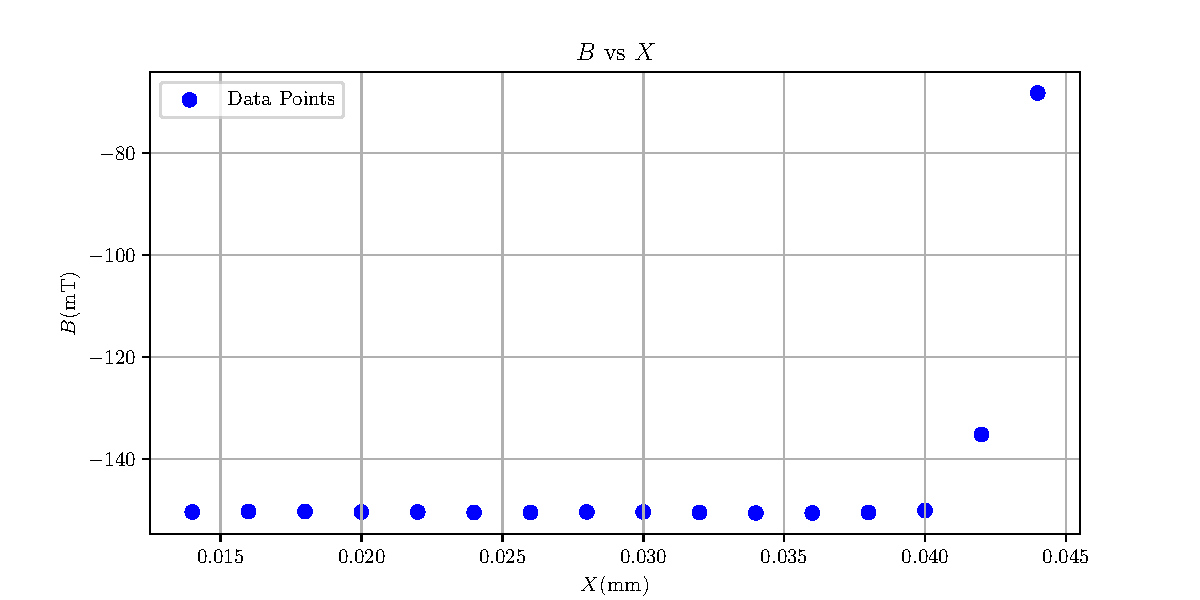
\includegraphics[width=0.8\textwidth]{plot5.pdf}
    \caption{电磁铁磁场沿水平方向分布}
\end{figure}
可以观察到电磁铁磁场在超出一定距离后迅速下降

\begin{table}[H]
\centering
\begin{tabular}{|c|c|c|c|c|c|c|c|} 
\hline
$I_M(\mathrm{mA})$ & 50    & 75    & 100   & 125   & 150   & 175   & 200    \\ 
\hline
$B(\mathrm{mT})$ & 38.0  & 57.1  & 75.4  & 94.4  & 113.3 & 131.6 & 150.5  \\ 
\hline
$V_{H-\mathrm{AC}}(\mathrm{mV})$ & 13.80 & 20.68 & 27.56 & 34.35 & 41.08 & 47.92 & 54.72  \\
\hline
\end{tabular}
\caption{AC模式霍尔效应测量磁场, $I_{S-\mathrm{AC}} = 200\mathrm{mA}$}
\end{table}

利用最小二乘法进行线性拟合，绘制如下图像:

\begin{figure}[H]
    \centering
    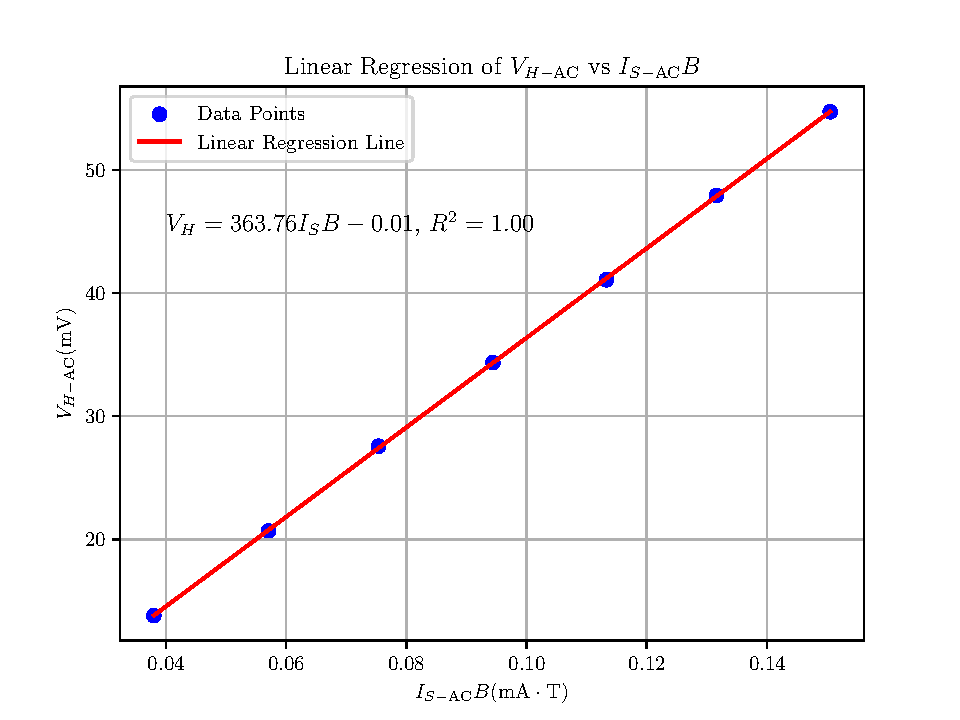
\includegraphics[width=0.8\textwidth]{plot6.pdf}
    \caption{AC模式霍尔效应测量磁场}
\end{figure}


可以得到$K_H = 363.76 \mathrm{V / A \cdot T}$, 和仪器标定值$K_H = 357 \mathrm{V / A \cdot T}$的误差相较于直流模式下的测量方式更大一些

\subsection{亥姆霍兹线圈磁感应强度测量}

\begin{table}[H]
\centering
\begin{tabular}{|c|c|c|c|c|c|c|c|c|c|c|c|} 
\hline
轴向距离 $X(\mathrm{mm})$ & -25   & -20   & -15   & -10   & -5    & 0     & 5     & 10    & 15    & 20  & 25   \\ 
\hline
$U_{\mathrm{max}} (\mathrm{mV})$ & 5.72  & 5.87  & 5.99  & 6.08  & 6.12  & 6.13  & 6.09  & 6.01  & 5.88  & 5.74  & 5.57  \\ 
\hline
$B_{\text{测}} = \tfrac{2.926}{f}U_{\mathrm{max}} (\mathrm{mT})$  & 0.139 & 0.143 & 0.146 & 0.148 & 0.149 & 0.149 & 0.148 & 0.147 & 0.143 & 0.140 & 0.136 \\ 
\hline
$B_{\text{理}}= \tfrac{\mu_0 N_0 I R^2}{2(R^2 + X^2)^{3/2}} (\mathrm{mT})$ & 0.130 & 0.135 & 0.138 & 0.141 & 0.143 & 0.144 & 0.143 & 0.142 & 0.140 & 0.138 & 0.134 \\
\hline
\end{tabular}
\caption{圆电流线圈轴线上磁场分布测量数据记录, $f=120\mathrm{Hz}$, $I = 60 \mathrm{mA}$, $N_0 = 400$, $R = 105\mathrm{mm}$}
\end{table}

使用二次多项式对测量数据以及理论数据进行拟合，绘制如下图像：

\begin{figure}[H]
    \centering
    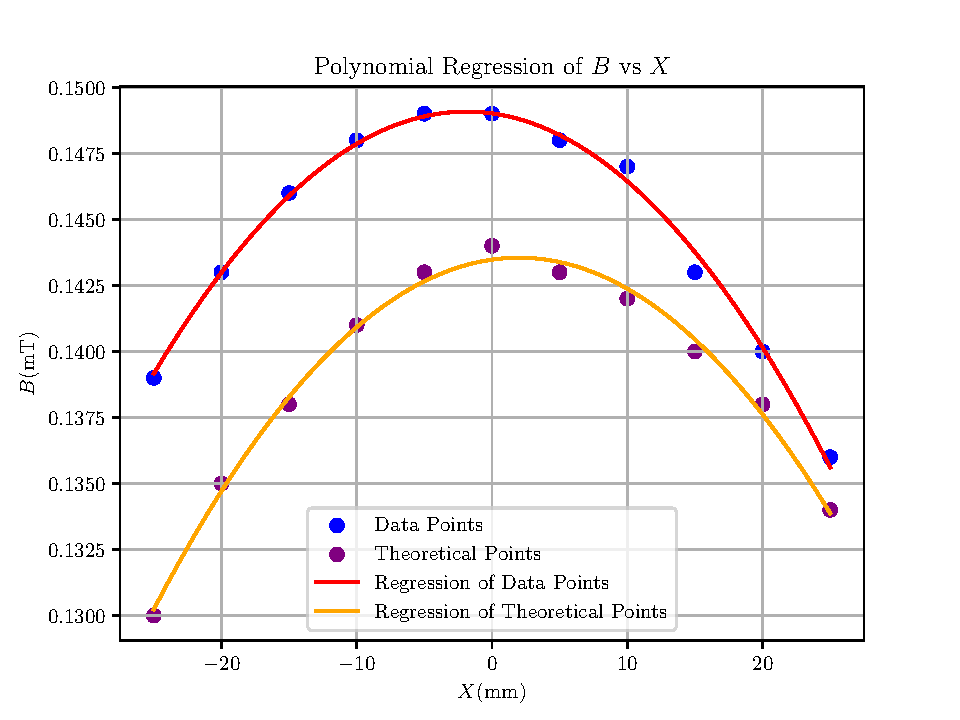
\includegraphics[width=0.8\textwidth]{plot7.pdf}
    \caption{圆电流线圈轴线上磁场分布}
\end{figure}

可以看出测量值与理论值具有相似的整体趋势, 但是测量值的峰值较理论值偏大

\begin{table}[H]
\centering
\begin{tabular}{|c|c|c|c|c|c|c|c|c|c|c|c|} 
\hline
轴向距离 $X(\mathrm{mm})$ & -25   & -20   & -15   & -10   & -5    & 0     & 5     & 10    & 15    & 20    & 25     \\ 
\hline
$U_{\mathrm{max}} (\mathrm{mV})$ & 8.74  & 8.74  & 8.75  & 8.75  & 8.75  & 8.75  & 8.75  & 8.76  & 8.76  & 8.75  & 8.74   \\ 
\hline
$B_{\text{测量}} = \tfrac{2.926}{f}U_{\mathrm{max}} (\mathrm{mT})$ & 0.213 & 0.213 & 0.213 & 0.213 & 0.213 & 0.213 & 0.213 & 0.214 & 0.214 & 0.213 & 0.213  \\
\hline
\end{tabular}
\caption{亥姆霍兹线圈轴线上磁场分布测量数据记录, $f=120\mathrm{Hz}$, $I = 60 \mathrm{mA}$}
\end{table}

作散点图如下
\begin{figure}[H]
    \centering
    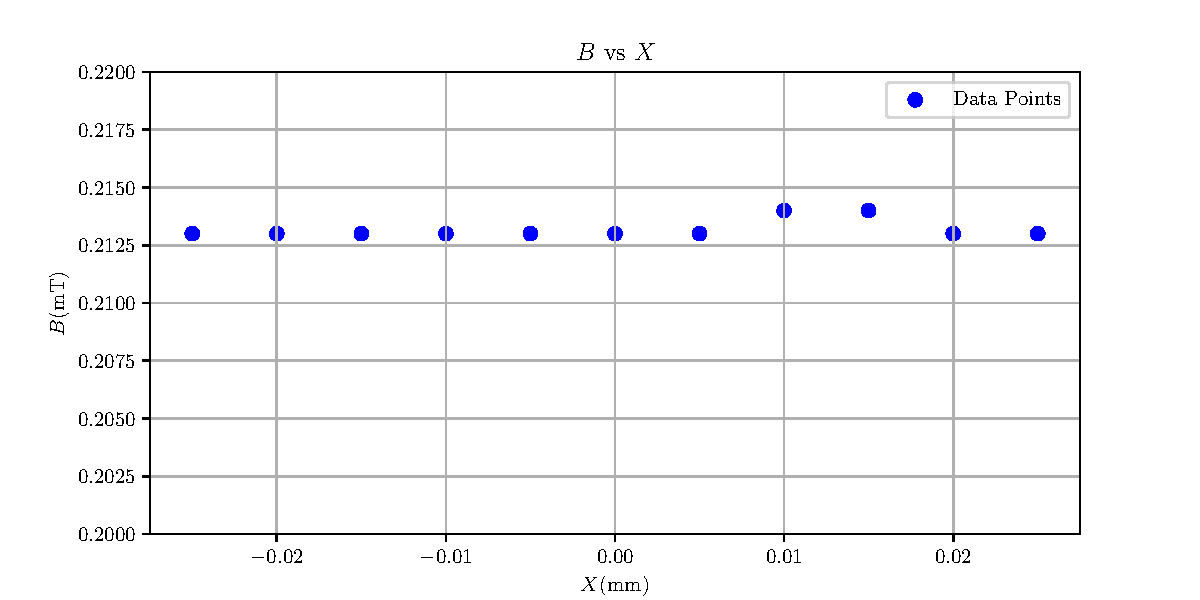
\includegraphics[width=0.8\textwidth]{plot8.pdf}
    \caption{亥姆霍兹线圈轴线上磁场分布}
\end{figure}

可以看出在轴向上磁感应强度有微小的涨落, 但是整体上保持不变

\begin{table}[H]
\centering
\begin{tabular}{|c|c|c|c|c|c|c|c|c|c|c|c|} 
\hline
径向距离 $X(\mathrm{mm})$ & -25   & -20   & -15   & -10   & -5    & 0     & 5     & 10    & 15    & 20    & 25     \\ 
\hline
$U_{\mathrm{max}} (\mathrm{mV})$ & 8.69  & 8.70  & 8.71  & 8.71  & 8.71  & 8.71  & 8.70  & 8.70  & 8.70  & 8.69  & 8.67   \\ 
\hline
$B_{\text{测量}} = \tfrac{2.926}{f}U_{\mathrm{max}} (\mathrm{mT})$ & 0.212 & 0.212 & 0.212 & 0.212 & 0.212 & 0.212 & 0.212 & 0.212 & 0.212 & 0.212 & 0.211  \\
\hline
\end{tabular}
\caption{亥姆霍兹线圈磁场径向分布测量数据记录, $f=120\mathrm{Hz}$, $I = 60 \mathrm{mA}$}
\end{table}

也作散点图如下

\begin{figure}[H]
    \centering
    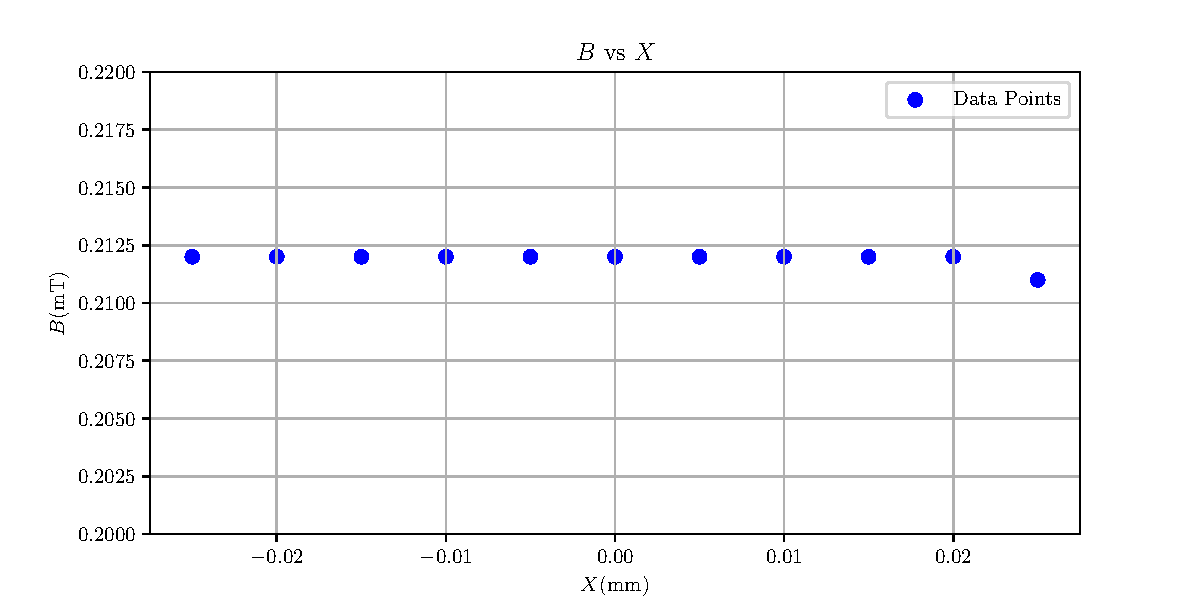
\includegraphics[width=0.8\textwidth]{plot9.pdf}
    \caption{亥姆霍兹线圈磁场径向分布}
\end{figure}


可以看出在径向上磁感应强度几乎保持稳定不变

\begin{table}[H]
\centering
\begin{tabular}{|c|c|c|c|c|c|c|c|c|c|c|} 
\hline
探测线圈转角$\theta$     & 0    & 10   & 20   & 30   & 40   & 50   & 60   & 70   & 80   & 90    \\ 
\hline
$U_{\text{测量}} (\mathrm{mV})$         & 8.71 & 8.56 & 8.18 & 7.58 & 6.70 & 5.52 & 4.15 & 2.75 & 1.37 & 0.00  \\ 
\hline
$U_{\text{理论}} = U_{\mathrm{max}} \cos \theta$ & 8.71 & 8.58 & 8.18 & 7.54 & 6.67 & 5.60 & 4.36 & 2.98 & 1.51 & 0.00  \\ 
\hline
探测线圈转角$\theta$     & 100  & 110  & 120  & 130  & 140  & 150  & 160  & 170  & 180  & 190   \\ 
\hline
$U_{\text{测量}} (\mathrm{mV})$         & 1.63 & 3.05 & 4.30 & 5.65 & 6.66 & 7.54 & 8.14 & 8.53 & 8.66 & 8.55  \\ 
\hline
$U_{\text{理论}} = U_{\mathrm{max}} \cos \theta$ & 1.51 & 2.98 & 4.36 & 5.60 & 6.67 & 7.54 & 8.18 & 8.58 & 8.71 & 8.58  \\ 
\hline
探测线圈转角$\theta$     & 200  & 210  & 220  & 230  & 240  & 250  & 260  & 270  & 280  & 290   \\ 
\hline
$U_{\text{测量}} (\mathrm{mV})$         & 8.17 & 7.59 & 6.82 & 5.76 & 4.17 & 2.76 & 1.27 & 0.00 & 1.76 & 3.17  \\ 
\hline
$U_{\text{理论}} = U_{\mathrm{max}} \cos \theta$ & 8.18 & 7.54 & 6.67 & 5.60 & 4.36 & 2.98 & 1.51 & 0.00 & 1.51 & 2.98      \\ 
\hline
探测线圈转角$\theta$     & 300  & 310  & 320  & 330  & 340  & 350  & 360  &      &      &       \\ 
\hline
$U_{\text{测量}} (\mathrm{mV})$         & 4.56 & 5.72 & 6.76 & 7.59 & 8.19 & 8.59 & 8.71 &      &      &       \\ 
\hline
$U_{\text{理论}} = U_{\mathrm{max}} \cos \theta$ & 4.36 & 5.60 & 6.67 & 7.54 & 8.18 & 8.58 & 8.71 &      &      &       \\
\hline
\end{tabular}
\caption{探测线圈转角与感应电压之间的关系数据记录, $f=120\mathrm{Hz}$, $I = 60 \mathrm{mA}$}
\end{table}

使用Fourier级数对测量数据进行拟合，绘制如下图像：

\begin{figure}[H]
    \centering
    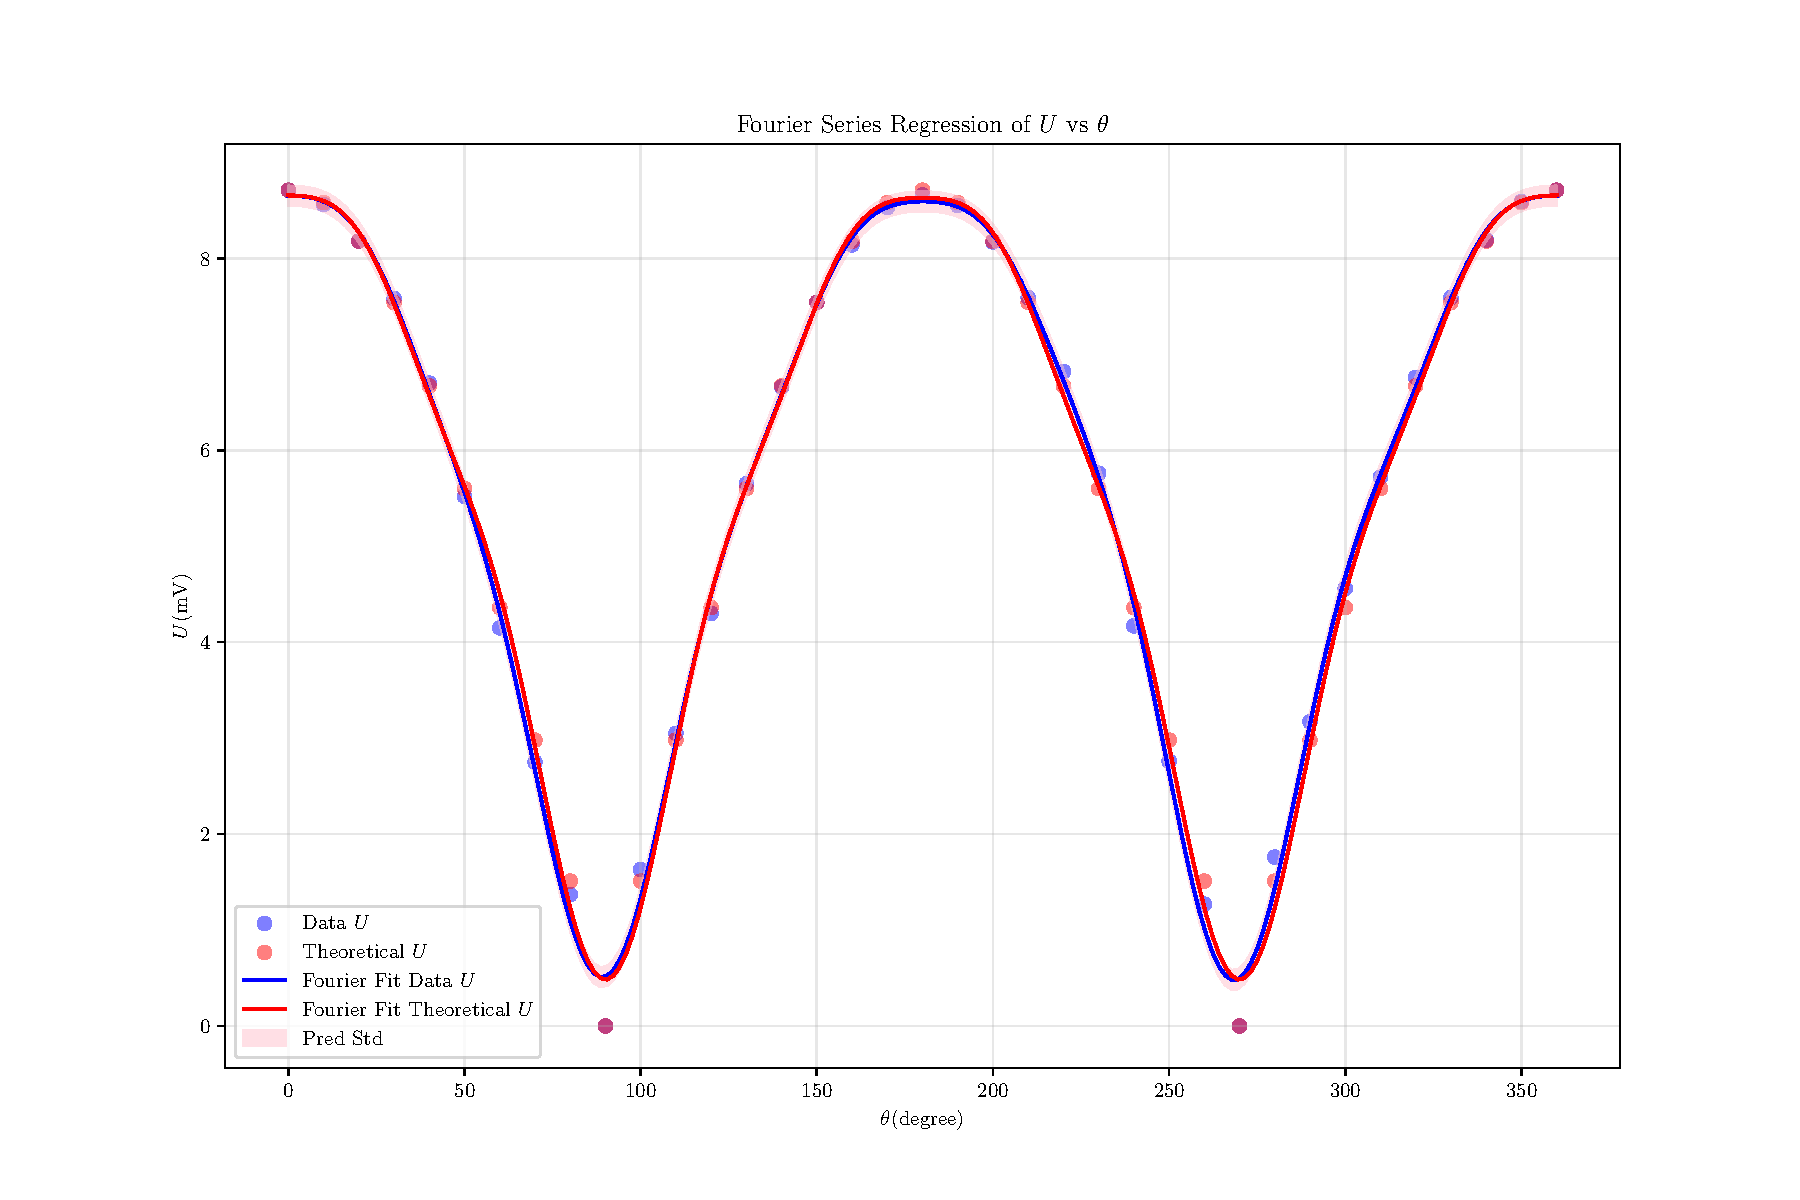
\includegraphics[width=0.8\textwidth]{plot10.pdf}
    \caption{探测线圈转角与感应电压之间的关系}
\end{figure}

可以发现测量值与理论值基本相同，由于实验数据中记录的是$B$的大小，所以整体数据呈现绝对值余弦函数的形状
\begin{table}[H]
\centering
\begin{tabular}{|c|c|c|c|c|c|c|c|c|c|c|c|} 
\hline
励磁电流频率$f(\mathrm{Hz})$ & 20    & 30    & 40    & 50    & 60    & 70    & 80    & 90    & 100   & 110   & 120    \\ 
\hline
$U_{\mathrm{max}}(\mathrm{mV})$ & 1.45  & 2.18  & 2.9   & 3.63  & 4.35  & 5.07  & 5.8   & 6.52  & 7.25  & 7.97  & 8.71   \\ 
\hline
$B_{\text{测量}} = \tfrac{2.926}{f}U_{\mathrm{max}} (\mathrm{mT})$ & 0.212 & 0.213 & 0.212 & 0.212 & 0.212 & 0.212 & 0.212 & 0.212 & 0.212 & 0.212 & 0.212  \\
\hline
\end{tabular}
\caption{励磁电流频率变化对于磁场强度的影响数据记录, $I = 60 \mathrm{mA}$}
\end{table}

作散点图如下
\begin{figure}[H]
    \centering
    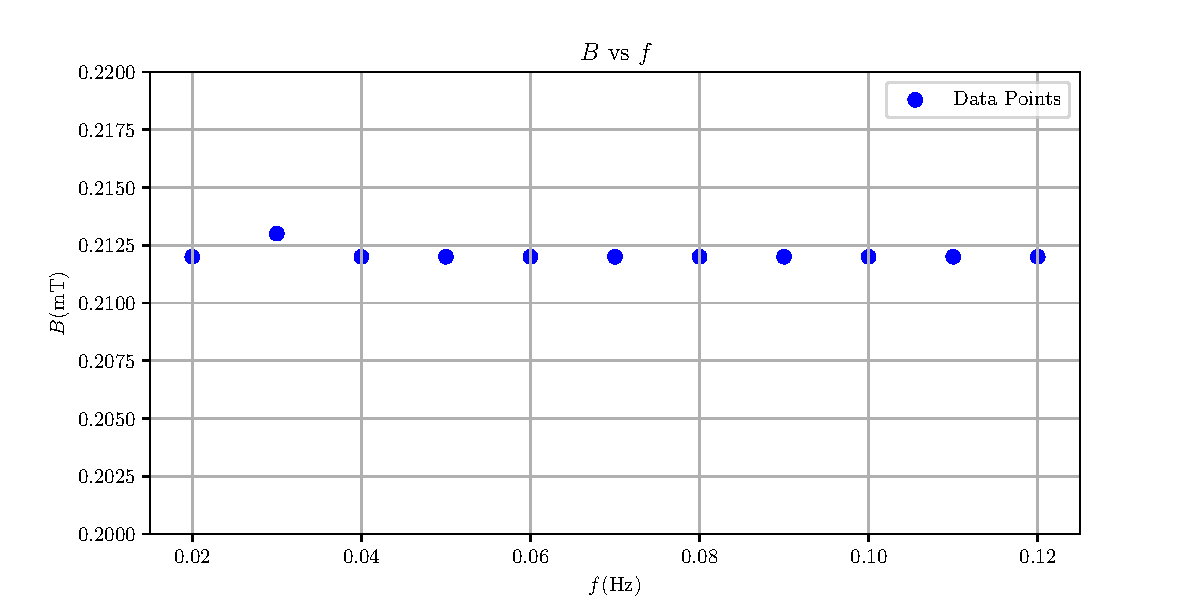
\includegraphics[width=0.8\textwidth]{plot11.pdf}
    \caption{励磁电流频率变化对于磁场强度的影响}
\end{figure}

可以发现发实验误差范围内,磁场强度几乎不随励磁电流频率发生变化

\section{讨论}
\subsection{实验总结}
\subsubsection{霍尔效应测量磁感应强度}
本次实验验主要使用 DH4512D 霍尔效应实验仪进行实验, 大量的实验细节已经被试验仪封装好，总体操作较为简单直观。实验过程中需要注意励磁电流和霍尔元件工作电流的能量源不能接反，否则将烧坏霍尔元件。在实验开始之前，要注意把电流输出调零，并且使得霍尔元件处在电磁铁中心位置；实验结束后，也要记得先将电源输出调零再关闭机器

实验得到的结果大多呈现良好的线性，且计算出的霍尔灵敏系数和标定值差距不大，说明该实验的精度是比较高的。但是在实验中，我们发现在测量霍尔灵敏度时，直流模式下的测量结果比交流模式下的测量结果更接近标定值，这可能是因为直流模式下的测量更加稳定，而交流模式下的测量一方面可能是实验电路更加复杂引入误差的因素增多，或者是受到了电流频率的影响，导致了测量结果的偏差。

另外，在交流模式下测量磁场时，在搭建完实验电路后需要先向老师确认后再开启电源，以免误接造成的短路等问题损坏实验仪器。

\subsubsection{亥姆霍兹线圈磁感应强度测量}
在测量圆形电流线圈的磁场时，要注意传感器位置$X$的零点要设在通电线圈的中心，实际操作中线圈中心的位置难以有精确的标定，不过我们也可以从测量数据的曲线来反推线圈中心的位置。在测量亥姆霍兹线圈的磁场时，我们发现在轴向上磁感应强度有微小的涨落，但是整体上保持不变；在径向上磁感应强度几乎保持稳定不变，这说明亥姆霍兹线圈的磁场是比较均匀的。

在旋转传感器线圈的时候，可能会被一些螺丝挡住某些角度的示数，这时候可以以另一边的示数作为参考，或者是将螺丝拧下来，再将其拧回去（虽然我们没有尝试过）。以及由于余弦曲线的性质，在极值中间角度范围，示数变化较大，我认为这里可以减小角度的间隔，以提高测量的精度。
\subsection{心得}
\begin{enumerate}
    \item 做实验的时候，首先要保证人身安全，其次要保证仪器的安全。在实验过程中，要注意实验仪器的使用方法，在进行一些关键的操作比如说通电、调节信号幅值的时候，要先确认无误后再进行操作，以免损坏仪器。
    \item 在实验的过程中，对于记录有误的数据，或者因为实验失误而导致的数据不准确，不需要马上删除，可以先记录下来，等到实验结束后再进行筛选，这样一方面可以保证数据的完整性，另一方面也有助于找出实验中容易出现问题的环节，从而为下一次实验做准备。
    \item 一些实验中的细节被高度封装的仪器系统所掩盖了，这虽然方便了实验的进行，但是也容易让人无法对整个实验的过程有个全面的把握，所以在实验结束后，可以尝试对实验的原理进行一些推导，或者是对实验的细节进行一些思考，了解这些实验仪器实际上帮助我们做了说明书，这样可以更好地理解实验的原理，也有助于对实验的结果进行分析。
\end{enumerate}
\section{思考题}
\subsection{霍尔效应测量磁感应强度}
\textbf{分析本实验主要误差来源, 计算磁感应强度$B$的合成不确定度, 分别取$I_M = 0.2\mathrm{A}, I_H = 1\mathrm{mA}$}

本实验主要误差来源有以下几点：
\begin{enumerate}
    \item 霍尔元件本身的误差，包括霍尔元件的灵敏度$K_H$的误差，以及霍尔元件的位置误差
    \item 霍尔元件带来的各种副效应造成的误差，尤其是爱廷豪森效应带来的干扰
    \item 电路中的各种元件的误差，包括电源的稳定性，电流源的示数误差等
\end{enumerate}
计算磁感应强度$B$的合成不确定度:
\[
\begin{aligned}
B &= U_H / K_H I_H \\
\implies u(B)^2 &= \left[\frac{\partial B}{\partial U_H} u(U_H)\right]^2 + \left[\frac{\partial B}{\partial K_H} u(K_H)\right]^2 + \left[\frac{\partial B}{\partial I_H} u(I_H)\right]^2
\end{aligned}
\]
由此可计算得$u(B) = 0.5 \mathrm{mT}$

\textbf{以简图示意,用霍尔效应法判断霍尔片上磁感应强度方向}

在下图中如果霍尔元件左边的电势高，则磁场向上; 如果右边的电势高，则磁场向下
\begin{figure}[H]
    \centering
    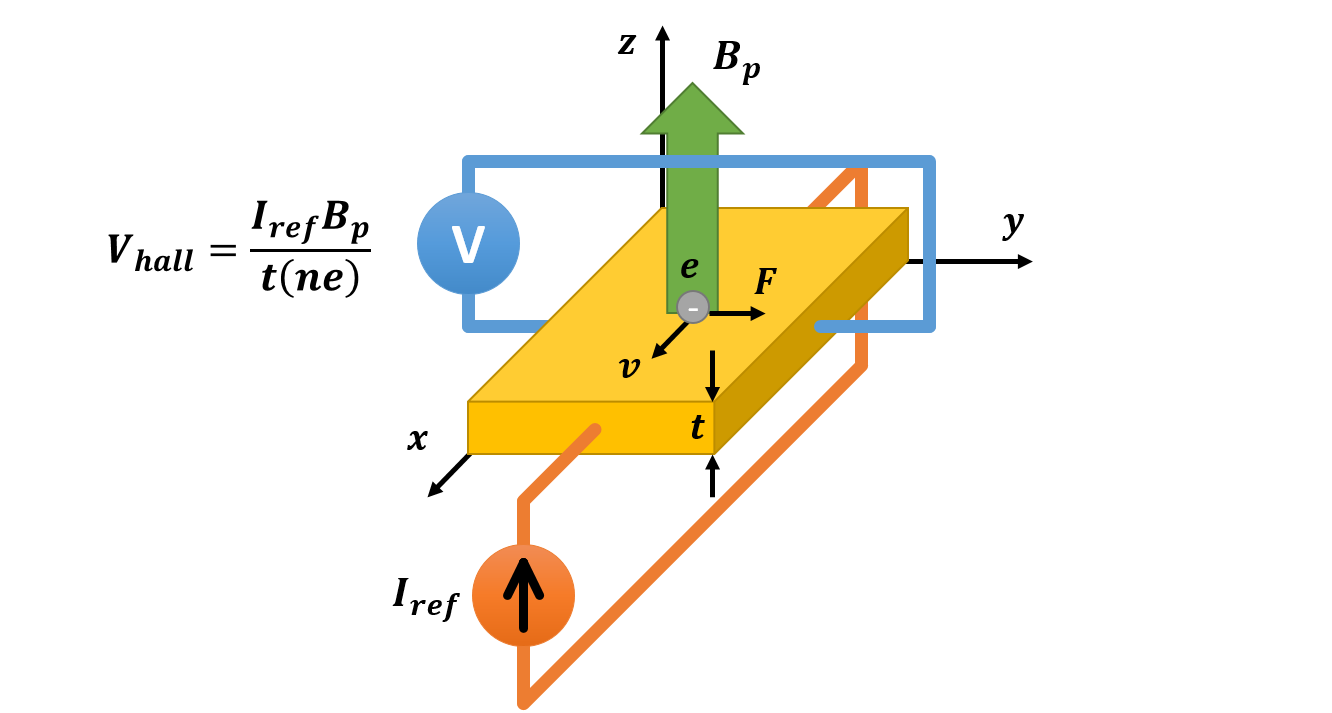
\includegraphics[width=0.8\textwidth]{Hall-effect.png}
    \caption{霍尔效应法判断磁感应强度方向}
\end{figure}

\textbf{如何测量交变磁感应强度, 写出主要步骤}

\begin{enumerate}
    \item 在已知的静态磁场下对霍尔传感器进行校准，以确保输出电压与磁场强度之间的关系准确
    \item 将霍尔元件放置在待测交变电场的适当位置，确保其敏感面与电场方向垂直，以便准确捕捉到交变磁场
    \item 通过施加交变电流到导体中，产生交变电场。确保频率和幅度在霍尔元件的测量范围内
    \item 观察并记录霍尔元件输出的电压信号，使用示波器可以更清晰地看到信号的波形和变化
\end{enumerate}
\subsection{亥姆霍兹线圈磁感应强度测量}
\textbf{单线圈轴线上磁场的分布规律如何？亥姆霍兹线圈是怎样组成的？其基本条件有哪些？它的磁场分布特点怎样？}
\begin{enumerate}
    \item 对于半径为$R$的圆线圈，通以电流$I$，在距离线圈中心$X$处的磁感应强度$B(X)$可以通过以下公式表示：
\[
B(X) = \frac{\mu_0 N I R^2}{2(R^2 + X^2)^{3/2}}
\]
其中，$\mu_0$是真空中的磁导率，$N$是线圈的匝数。可以看出，随着距离$X$的增加，磁感应强度$B(X)$会逐渐减小，并且在轴线上呈现出对称分布的特性。
    \item 亥姆霍兹线圈由两个相同的圆形线圈组成，这两个线圈彼此平行且共轴，间距等于它们的半径$R$。每个线圈都通以相同方向和大小的电流
    \item 两个线圈必须具有相同的半径$R$; 两个线圈的匝数$N$应相同; 两条线圈中的电流方向必须一致，以确保在共同轴线上产生叠加效应; 两线圈之间的距离必须等于其半径，以确保最佳的均匀性
    \item 亥姆霍兹线圈在其中心区域能够产生非常均匀的磁场
\end{enumerate}

\textbf{探测线圈放入磁场后，不同方向上毫伏表指示值不同，哪个方向最大？如何测准$U_\mathrm{max}$值？指示值最小表示什么？}

当传感器线圈平面与磁感应强度方向垂直时，指示值最大，在0到360度之间扫描寻找最大值，这个过程中会出现两次最大值。如果两次出现最大值的相对偏差小于$2\%$，则取其中之一作为最大值，否则取二者平均值作为最大值，指示值最小表示测量线圈平面与磁感应强度方向平行

\textbf{分析圆电流磁场分布的理论值与实验值的误差的产生原因}

\begin{enumerate}
    \item 线圈的中心位置难以准确标定，导致实际测量的位置与理论值有一定的偏差
    \item 电压表没有调零，导致了系统误差
    \item 周围环境对于磁场的干扰，比如说铁磁材料等
\end{enumerate}
\subsection{同学留下的一道思考题}
上一位同学留下的思考题是：\textbf{实验中导致误差的因素有哪些}. 霍尔元件和单线圈的误差因素上面已经提过了，所以这里列举一些亥姆霍兹线圈的误差因素：
\begin{enumerate}
    \item 传感线圈本身的误差，包括线圈的灵敏度$K$的误差，以及线圈的位置误差（传感器的中心真的和下面刻度的标定示数一致吗?）
    \item 电流源的稳定性，电流源的示数误差等
    \item 转动线圈时候角度的读数误差
\end{enumerate}
\section{附录}
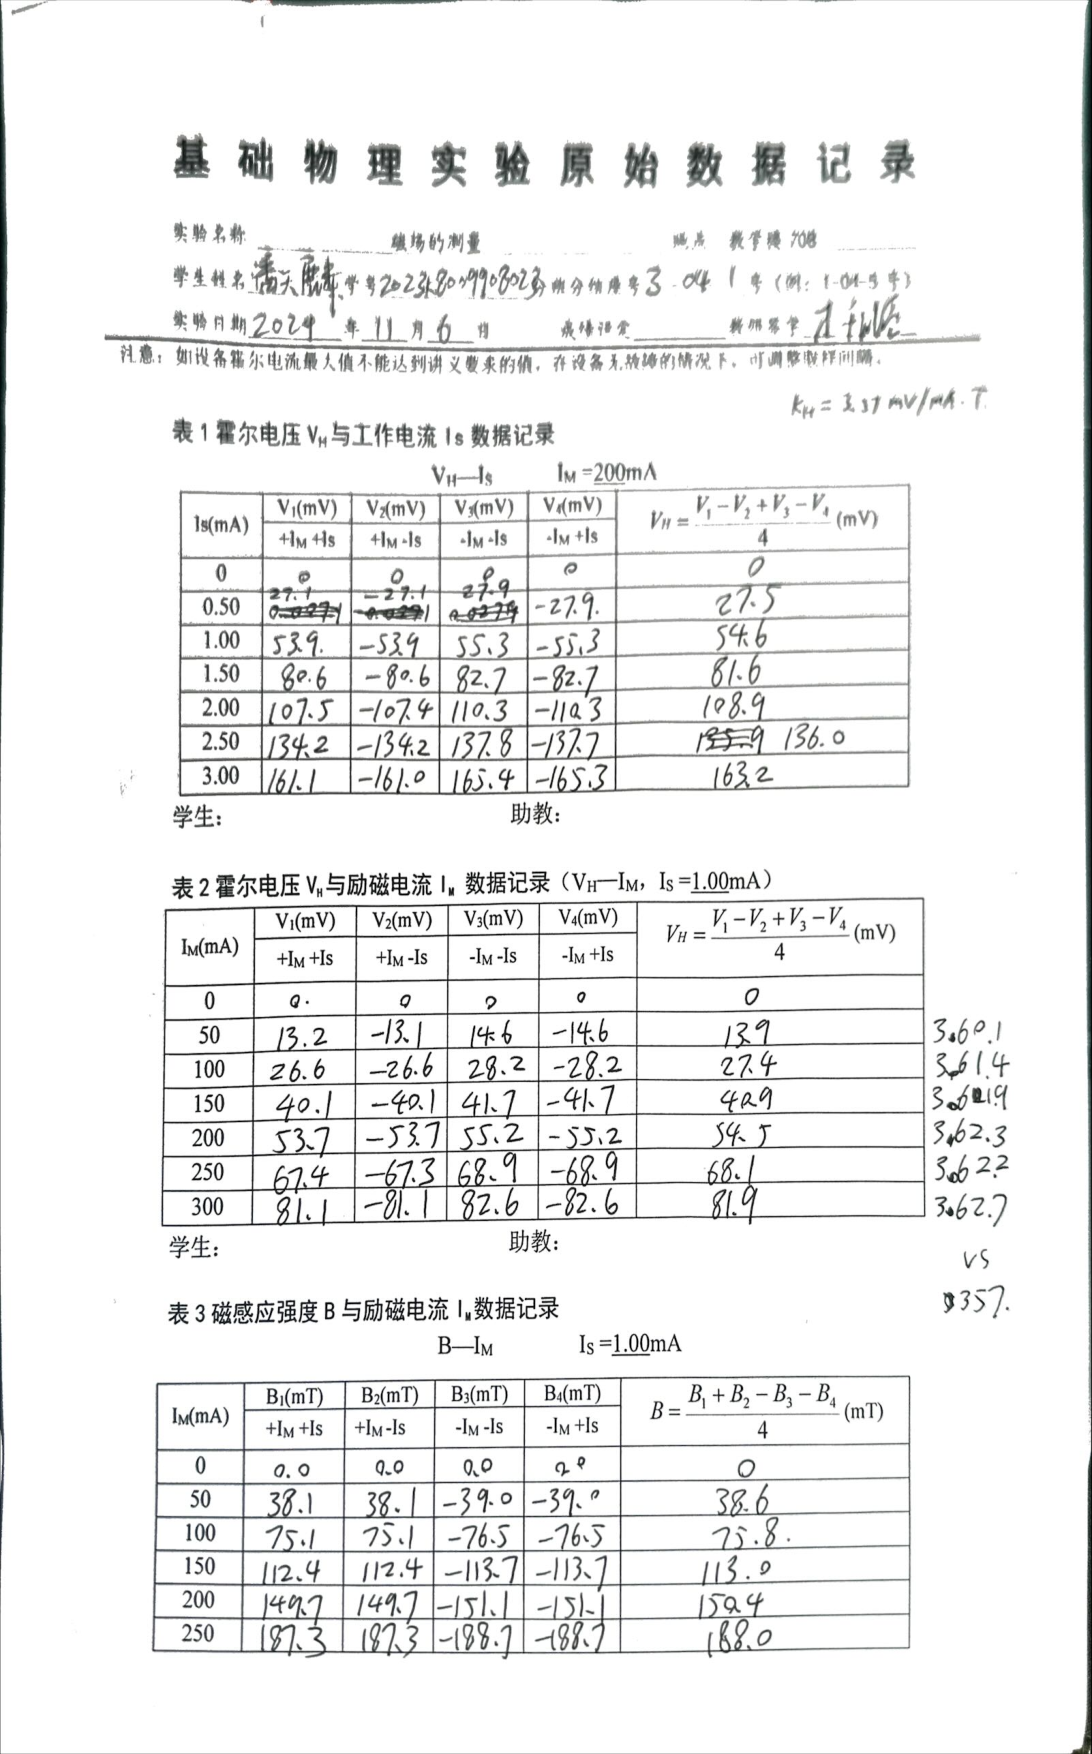
\includepdf[pages=-]{潘天麟-磁场测量-数据.pdf}
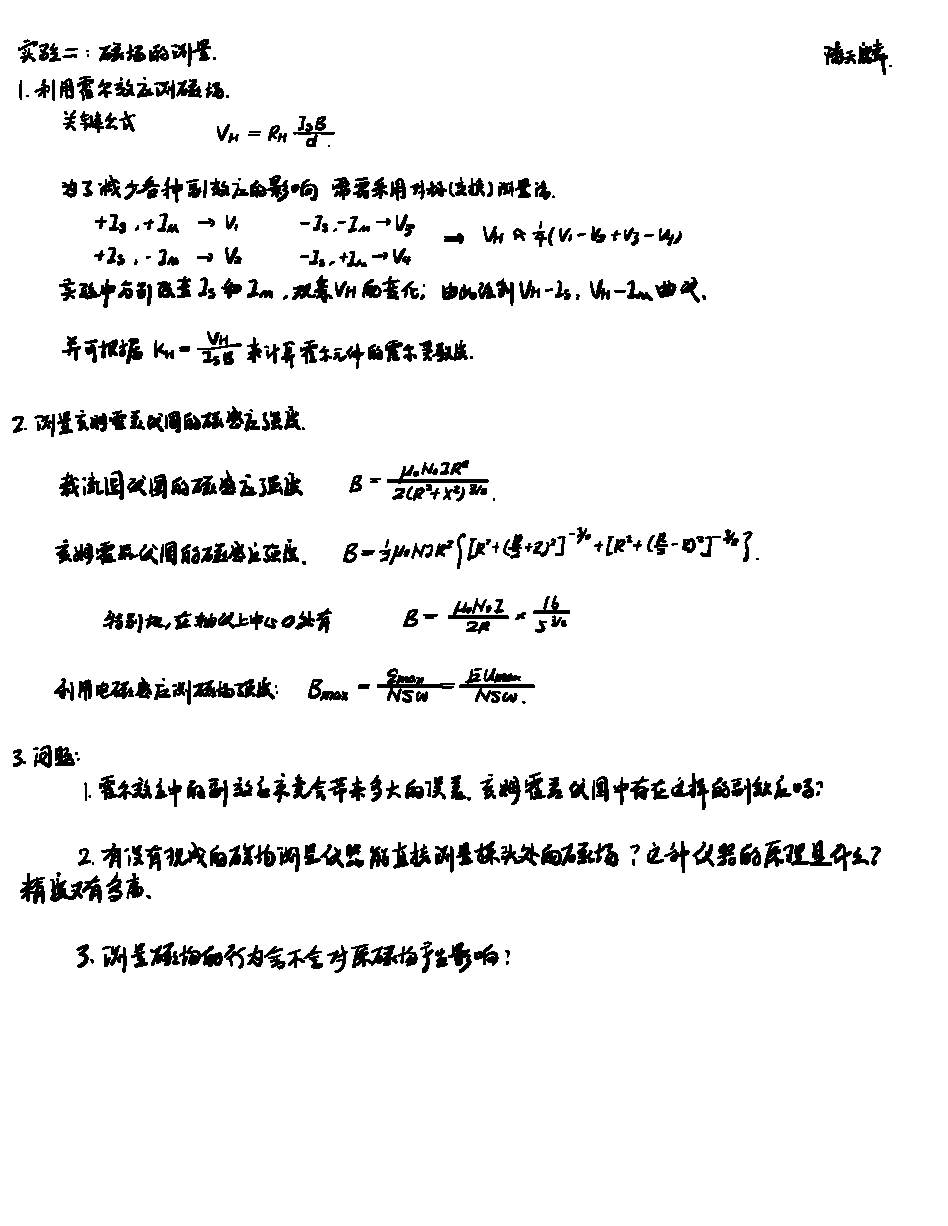
\includepdf[pages=-]{潘天麟-2024-11-6-磁场测量-预习报告.pdf}
\end{document}
